\documentclass{article}
\usepackage{amsmath}
\usepackage[margin=1in]{geometry}
\usepackage{amsfonts}
\usepackage{hyperref}
\usepackage{graphicx}

\begin{document}
	
\title{Linear Combination}
\author{Andy Chong Sam}

\maketitle	

\section{Linear Combinations Visual Intuition}
\begin{minipage}[c]{.5\linewidth}
	\par \noindent We first start with the idea of a generic vector which can be scaled by a positive or negative k. As seen on Figure 1, scaling the vector positively or negatively through \(k\) will result in a line.
\end{minipage}%%%
\begin{minipage}[c]{.5\linewidth}
\begin{center}
	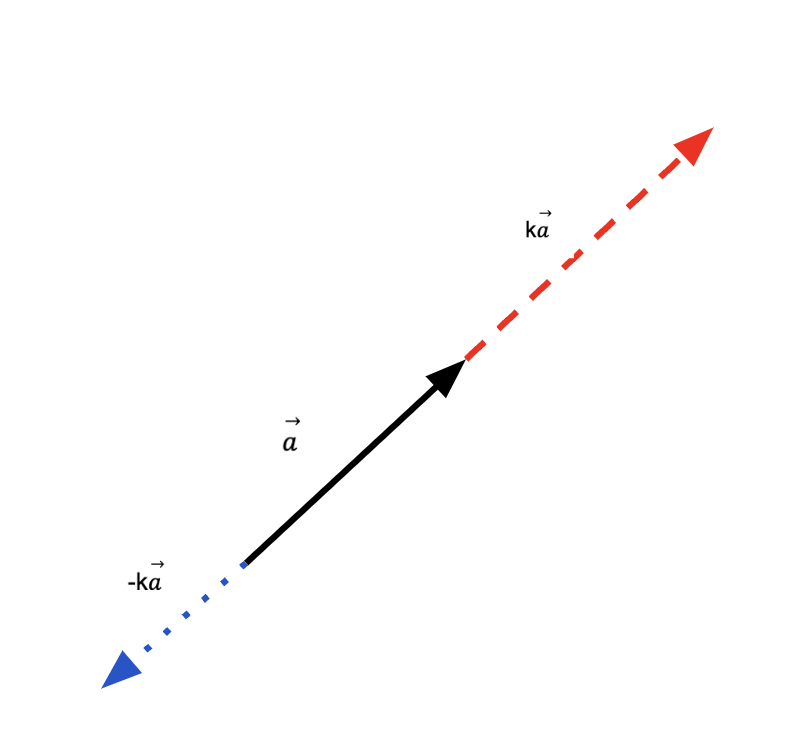
\includegraphics[width=3cm]{matrix-scaling-1.png}
\end{center}
\begin{center}
	Figure 1	
\end{center}
\end{minipage}
\linebreak
\linebreak
\linebreak
\begin{minipage}[c]{.5\linewidth}
	\par \noindent Now suppose we have two vectors \( \vec a \) and \( \vec b \).  They can each be scaled independently. Both vectors can also be added together. With some visual imagination we can see that by varying the scaling factor of each vector we can reach every point on the two dimensional plane.
\end{minipage}%%%
\begin{minipage}[c]{.5\linewidth}
\begin{center}
	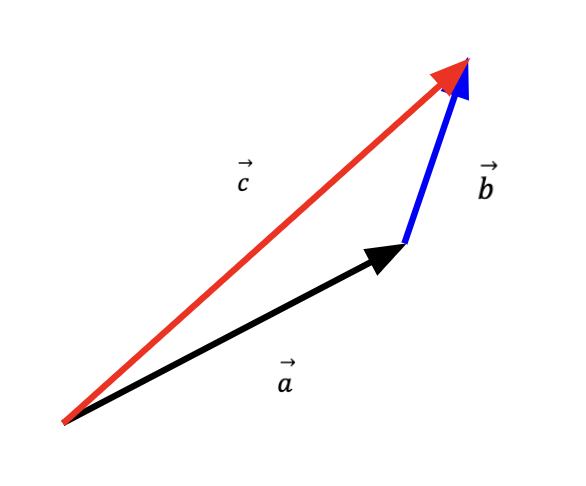
\includegraphics[width=3cm]{vector-scaling-2.png}
\end{center}
\begin{center}
	Figure 2	
\end{center}
\end{minipage}
\linebreak
\linebreak
\linebreak
\begin{minipage}[c]{.5\linewidth}
	\par \noindent We can of course add multiple vectors together, each with the ability to scale independently. A hypothetical situation with three vectors is shown on Figure 3.
\end{minipage}%%%
\begin{minipage}[c]{.5\linewidth}
\begin{center}
	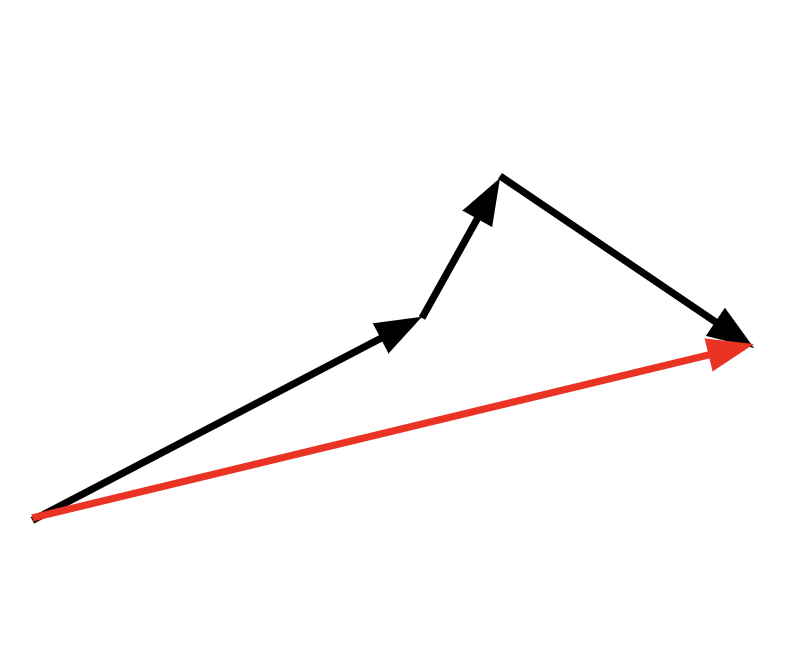
\includegraphics[width=3cm]{matrix-scaling-3.png}
\end{center}
\begin{center}
	Figure 3
\end{center}
\end{minipage}
\newline
\newline
\newline
\par\noindent The points that can be reached by adding and scaling a set of vectors is the \textbf{span} of the vector set. The set of vectors themselves (along with any scaling and vector addition) is referred to as a \textbf{vector space}.
\newpage
\par \noindent We can describe the summation and scaling of n vectors \(<x_n, y_n>\) together like so:
\newline
\[
k_1
\left(\begin{array}{@{}c@{}}
	x_1 \\
	y_1 \\
\end{array}\right) + 
k_2
\left(\begin{array}{@{}c@{}}
	x_2 \\
	y_2 \\
\end{array}\right) + 
k_3
\left(\begin{array}{@{}c@{}}
	x_3 \\
	y_3 \\
\end{array}\right) + 
... 
k_n
\left(\begin{array}{@{}c@{}}
	x_n \\
	y_n \\
\end{array}\right) =
\left(\begin{array}{@{}c@{}}
	k_1 x_1 + k_2 x_2 + k_3 x_3... + k_n x_n \\
	k_1 y_1 + k_2 y_2 + k_3 y_3... + k_n y_n \\
\end{array}\right) 
\]
\newline
\par \noindent The expression above can be rewritten in the form of a matrix multiplication:
\newline
\[
\left(\begin{array}{@{}ccccc@{}}
	x_1 & x_2 & x_3 &... &x_n\\
	y_1 & y_2 & y_3 & ... &y_n\\
	
\end{array}\right) 
\left(\begin{array}{@{}c@{}}
	k_1 \\
	k_2 \\
	k_3 \\
	... \\
	k_n
\end{array}\right) 
\]
\newline
\par \noindent It is for this reason that when vectors are written into a matrix they are often done so vertically down a column.
\newline
\par \noindent With this in mind, we can document two important vector spaces, \(\mathbb{R}^2\)  and \(\mathbb{R}^3\).Consider the following linear combination:
\newline
\[
k_1
\left(\begin{array}{@{}c@{}}
	1 \\
	0 \\
\end{array}\right) + 
k_2
\left(\begin{array}{@{}c@{}}
	0 \\
	1 \\
\end{array}\right)
\]
\newline
\par \noindent We can visualize how any point on the two dimensional coordinate plane can be reached by simply adjusting the values for \(k_1\) and \(k_2\). This is the vector space known as \( \mathbb{R}^2 \). Now consider the following combination:
\newline
\[
k_1
\left(\begin{array}{@{}c@{}}
	1 \\
	0 \\
	0 
\end{array}\right) + 
k_2
\left(\begin{array}{@{}c@{}}
	0 \\
	1 \\
	0
\end{array}\right) +
k_3
\left(\begin{array}{@{}c@{}}
	0 \\
	0 \\
	1
\end{array}\right)
\]
\newline
\par \noindent By adjusting the values for \(k_1\), \(k_2\) and \(k_3\) we can reach every point in the three dimensional coordinate system. This vector space is known as \(\mathbb{R}^3\).


\newpage
\par \noindent Problems related to linear combinations involve verifying if a vector is a combination of other vectors. A few examples are provided below.
\newline
\newline
\framebox{
	\parbox{\linewidth}
	{
		\par\noindent Write \(<10,12>\) as a linear combination of \(<2,2>\) and \(<3,1>\).
		\newline
		\par\noindent We want to solve for the matrix \(<k_1, k_2>\):
		\[
			\left(\begin{array}{@{}cc@{}}
				2 & 3\\
				2 & 1\\
			\end{array}\right) 
			\left(\begin{array}{@{}c@{}}
				k_1\\
				k_2\\
			\end{array}\right) =
			\left(\begin{array}{@{}c@{}}
				10\\
				12\\
			\end{array}\right)	
		\]
		\par\noindent Which can be solved with the augmented matrix:
		\[
			\left(\begin{array}{@{}cc|c@{}}
				2 & 3 & 10\\
				2 & 1 & 12\\
			\end{array}\right) 
		\]
		\[
			\left(\begin{array}{@{}cc|c@{}}
				2 & 3 & 10\\
				2 & 1 & 12\\
				\end{array}\right)
			\xrightarrow[]{R_2 - R_1 = R_2} 	
			\left(\begin{array}{@{}cc|c@{}}
				2 & 3 & 10\\
				0 & -2 & 2\\
			\end{array}\right)	
			\xrightarrow[]{-\frac{1}{2}R_2 = R_2} 
			\left(\begin{array}{@{}cc|c@{}}
				2 & 3 & 10\\
				0 & 1 & -1\\
			\end{array}\right)		
			\xrightarrow[]{-\frac{1}{2}R_1 = R_1}							
		\]
		\[
		\left(\begin{array}{@{}cc|c@{}}
			1 & \frac{3}{2} & 5\\
			0 & 1 & -1\\
		\end{array}\right)
		\xrightarrow[]{R_1 - \frac{3}{2}R_2 = R_1}	
			\left(\begin{array}{@{}cc|c@{}}
			1 & 0 & \frac{13}{2}\\
			0 & 1 & -1\\
			\end{array}\right)		
		\]
		\newline
		\par\noindent \textbf{Solution:}
		\[
		 \frac{13}{2}
		\left(\begin{array}{@{}c@{}}
			2 \\
			2 \\
		\end{array}\right) -
		\left(\begin{array}{@{}c@{}}
		3 \\
		1 \\
		\end{array}\right)		
		=
		\left(\begin{array}{@{}c@{}}
			10\\
			12\\
		\end{array}\right)\]
	}
}
\newline
\newline
\newline
\framebox{
	\parbox{\linewidth}
	{
		\par\noindent Write \(<-5,3,16>\) as a linear combination of \(<1, -1, 4>\) and \(<-3, 2, 6>\).
		\newline
		\par \noindent We proceed to setup the augmented matrix and reduce:
		\newline
		\[
		\left(\begin{array}{@{}cc|c@{}}
			1 & -3 & -5\\
			-1 & 2 & 3\\
			4 & 6 & 16 \\
		\end{array}\right)
		\xrightarrow[]{R_2 <--> R_3}	
		\left(\begin{array}{@{}cc|c@{}}
			1 & -3 & -5\\
			4 & 6 & 16 \\
		    -1 & 2 & 3\\
		\end{array}\right)
		\xrightarrow[]{\frac{1}{2}R_2 = R_2}	
		\left(\begin{array}{@{}cc|c@{}}
			1 & -3 & -5\\
			2 & 3 & 8 \\
			-1 & 2 & 3\\
		\end{array}\right)
		\xrightarrow[]{R_1 + R_2 = R_1}	
		\]
		\newline
		\[
		\left(\begin{array}{@{}cc|c@{}}
			3 & 0 & 3\\
			2 & 3 & 8\\
			-1 & 2 & 3 \\
		\end{array}\right)
		\xrightarrow[]{\frac{1}{3}R_1 = R_1}	
		\left(\begin{array}{@{}cc|c@{}}
			1 & 0 & 1\\
			2 & 3 & 8 \\
			-1 & 2 & 3\\
		\end{array}\right)
		\xrightarrow[]{R_2 - 2R_1 = R_2}	
		\left(\begin{array}{@{}cc|c@{}}
			1 & 0 & 1\\
			0 & 3 & 6 \\
			-1 & 2 & 3\\
		\end{array}\right)
		\xrightarrow[]{\frac{1}{3}R_2 = R_2}	
		\]
		\newline
		\[
		\left(\begin{array}{@{}cc|c@{}}
			1 & 0 & 1\\
			0 & 1 & 2\\
			-1 & 2 & 3 \\
		\end{array}\right)
		\xrightarrow[]{R_3 + R_1 = R_3}	
		\left(\begin{array}{@{}cc|c@{}}
			1 & 0 & 1\\
			0 & 1 & 2 \\
			0 & 2 & 4\\
		\end{array}\right)
		\xrightarrow[]{R_3 - 2R_2 = R_3}	
		\left(\begin{array}{@{}cc|c@{}}
			1 & 0 & 1\\
			0 & 1 & 2 \\
			0 & 0 & 0\\
		\end{array}\right)	
		\]
		\newline
		\par\noindent \textbf{Solution:} 
		\[
		\left(\begin{array}{@{}c@{}}
			1 \\
		   -1 \\
			4
		\end{array}\right) +
		2\left(\begin{array}{@{}c@{}}
			-3 \\
			2 \\
			6
		\end{array}\right)		
		=
		\left(\begin{array}{@{}c@{}}
			-5\\
			3\\
			16
		\end{array}\right)\]
}}
\newpage
\section{Linear Independence}
\par\noindent If a vector can be obtained by scaling another vector, then the two vectors are dependent. In a different case, suppose we have a set of three vectors. If one of the vectors can be derived by a combination of scaling and adding the other two vectors, then the set is also dependent. 
\newline
\par \noindent A set of vectors is dependent if there exists \( k_1 ... k_n\) such that \(k_1 \vec v_1 + ... k_n \vec v_n = 0\). If the only solution is the trivial solution \(k_1 = ... k_n = 0\), then the set is independent. 
\newline
\begin{minipage}[c]{.5\linewidth}
	\par \noindent Suppose we have \( \vec a = <1,1>\) and \( \vec b = <2,2>\) as shown on Figure 4. Since \( 2\vec a = \vec b\), the set \( \{ \vec a, \vec b\}\) is dependent.
\end{minipage}%%%
\begin{minipage}[c]{.5\linewidth}
	\begin{center}
		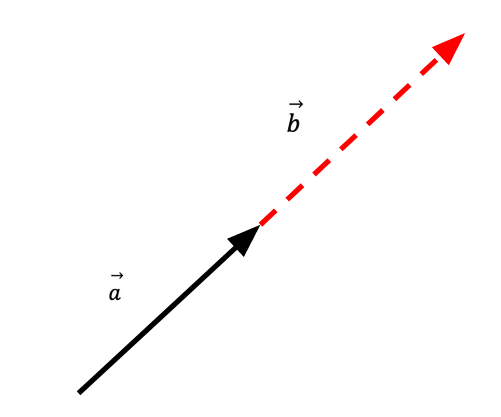
\includegraphics[width=3cm]{linear-combo.png}
	\end{center}
	\begin{center}
		Figure 4
	\end{center}
\end{minipage}
\newline
\par\noindent One possible intution is as follows. Suppose that there are two vectors \(v_1\) and \(v_2\). Based on our earlier definition, we know that if either vector can be scaled to obtain the other, then the set is not independent. If the set is dependent, then there is a constant \(k\) by which \(kv_2 = v_1\) or \(kv_1 = v_2\). In the latter case, we end up with \(kv_1 - v_2 = 0\). In this very specific example, the coefficient for \(v_2\) turned out to be negative, but we can generalize this whole expression to a general coefficient \(k_2\) which can be either positive or negative: \(k_1v_1 + k_2V_2 = 0\).
\newline
\par \noindent Here are some example problems:
\newline
\newline
\framebox{
	\parbox{\linewidth}
	{
	\par\noindent Determine if the set of vectors \(<2,2>\) and \(<-1,5>\) are independent or dependent.
	\newline
	\par\noindent We are solving for the matrix \(<k_1, k_2>\):
	\[
	\left(\begin{array}{@{}cc@{}}
		2 & -1 \\
		2 &  5 \\
	\end{array}\right)
\left(\begin{array}{@{}c@{}}
	k_1 \\
	k_2 \\
\end{array}\right)
	 = 
\left(\begin{array}{@{}c@{}}
	0 \\
	0 \\
\end{array}\right)	
\]
\[
	\left(\begin{array}{@{}cc|c@{}}
	2 & -1 & 0\\
	2 &  5 & 0 \\
\end{array}\right)
\xrightarrow[]{R_1 - \frac{1}{2}R_2 = R_1}
	\left(\begin{array}{@{}cc|c@{}}
	1 & -\frac{7}{2} & 0\\
	2 &  5 & 0 \\
\end{array}\right)
\xrightarrow[]{R_2 - 2R_1 = R_2}
	\left(\begin{array}{@{}cc|c@{}}
	2 & -\frac{7}{2} & 0\\
	0 &  12 & 0 \\
\end{array}\right)
\xrightarrow[]{\frac{1}{12}R_2 = R_2}
\]
\[
	\left(\begin{array}{@{}cc|c@{}}
	2 & -\frac{7}{2} & 0\\
	0 &  1 & 0 \\
\end{array}\right)
\xrightarrow[]{R_1 + \frac{7}{2}R_2 = R_1}
\left(\begin{array}{@{}cc|c@{}}
	2 &  0 & 0\\
	0 &  1 & 0 \\
\end{array}\right)
\xrightarrow[]{\frac{1}{2}R_1 = R_1}
\left(\begin{array}{@{}cc|c@{}}
	1 &  0 & 0\\
	0 &  1 & 0 \\
\end{array}\right)
\]
\[
\left(\begin{array}{@{}c@{}}
	k_1 \\
	k_2 \\
\end{array}\right) = 
\left(\begin{array}{@{}c@{}}
	0 \\
	0 \\
\end{array}\right)
\]
\par\noindent \textbf{The set is independent}.
}
}
\newline
\newline
\newline
\framebox{
	\parbox{\linewidth}
	{
		\par\noindent Determine if the set of vectors \(<-1,4>\) and \(<2,-8>\) are independent or dependent.
		\newline
		\par\noindent We are solving for the matrix \(<k_1, k_2>\):
		\[
		\left(\begin{array}{@{}cc@{}}
			-1 & 2 \\
			4 &  -8 \\
		\end{array}\right)
		\left(\begin{array}{@{}c@{}}
			k_1 \\
			k_2 \\
		\end{array}\right)
		= 
		\left(\begin{array}{@{}c@{}}
			0 \\
			0 \\
		\end{array}\right)	
		\]
		\[
		\left(\begin{array}{@{}cc|c@{}}
			-1 & 2 & 0\\
			4 &  -8 & 0 \\
		\end{array}\right)
		\xrightarrow[]{R_1 <--> R_2}
		\left(\begin{array}{@{}cc|c@{}}
			4 & -8 & 0\\
			-1 & 2 & 0 \\
		\end{array}\right)
		\xrightarrow[]{R_1 + 3R_2 = R_1}
		\left(\begin{array}{@{}cc|c@{}}
			1 & -2 & 0\\
			-1 & 2 & 0 \\
		\end{array}\right)
		\xrightarrow[]{R_2 + R_1 = R_2}
		\left(\begin{array}{@{}cc|c@{}}
			1 & -2 & 0\\
			0 &  0 & 0 \\
		\end{array}\right)
		\]		
		\par\noindent We are left with \(k_1 - 2k_2 = 0\), or \(k_1 = 2k_2\). Any combination of \(k_1\) and \(k_2\) that meet the established relationship will work, hence there are solutions other than the trivial solution.
		\newline
		\par\noindent \textbf{The set is dependent.}
	}
}
\newpage
\par\noindent Here are some examples using vectors with three components:
\newline
\framebox{
	\parbox{\linewidth}
	{
		\par\noindent Determine if the set of vectors \(<1,2,3>\) , \(<-2,1,0>\), and \(<1,0,1>\) are independent or dependent.
		\newline
		\par\noindent We are solving for the matrix \(<k_1, k_2, k_3>\):
		\[
			\left(\begin{array}{@{}ccc@{}}
				1 & -2 & 1 \\
				2 &  1 & 0 \\
				3 & 0 & 1 \\
			\end{array}\right)
			\left(\begin{array}{@{}c@{}}
				k_1 \\
				k_2 \\
				k_3 \\
			\end{array}\right)
			= 
			\left(\begin{array}{@{}c@{}}
				0 \\
				0 \\
				0 \\
			\end{array}\right)	
			\]	
			\[
			\left(\begin{array}{@{}ccc|c@{}}
				1 & -2 & 1 & 0\\
				2 &  1 & 0 & 0 \\
				3 & 0 & 1 & 0  \\
			\end{array}\right)
			\xrightarrow[]{R_2 - 2R_1 = R_2}
			\left(\begin{array}{@{}ccc|c@{}}
				1 & -2 & 1 & 0\\
				0 &  5 & -2 & 0 \\
				3 & 0 & 1 & 0  \\
			\end{array}\right)
			\xrightarrow[]{\frac{1}{5}R_2 = R_2}
			\left(\begin{array}{@{}ccc|c@{}}
				1 & -2 & 1 & 0\\
				0 &  1 & -\frac{2}{5} & 0 \\
				3 & 0 & 1 & 0  \\
			\end{array}\right)
			\xrightarrow[]{R_3 - 3R_1 = R_3}
			\]
			\[
			\left(\begin{array}{@{}ccc|c@{}}
				1 & -2 & 1 & 0\\
				0 &  1 & -\frac{2}{5} & 0 \\
				0 & 6 & -2 & 0  \\
			\end{array}\right)
			\xrightarrow[]{R_3 - 6R_2 = R_3}
			\left(\begin{array}{@{}ccc|c@{}}
				1 & -2 & 1 & 0\\
				0 &  1 & -\frac{2}{5} & 0 \\
				0 & 0 & \frac{2}{5} & 0  \\
			\end{array}\right)
		\xrightarrow[]{R_2+R_3=R_2}
			\left(\begin{array}{@{}ccc|c@{}}
			1 & -2 & 1 & 0\\
			0 &  1 & 0 & 0 \\
			0 & 0 & \frac{2}{5} & 0  \\
		\end{array}\right)
		\xrightarrow[]{R_1+2R_2=R_1} \\
			\]
			\[
			\left(\begin{array}{@{}ccc|c@{}}
		1 & 0 & 1 & 0\\
		0 &  1 & 0 & 0 \\
		0 & 0 & \frac{2}{5} & 0  \\
	\end{array}\right)
	\xrightarrow[]{\frac{5}{2}R_3 = R_3}
	\left(\begin{array}{@{}ccc|c@{}}
		1 & 0 & 1 & 0\\
		0 &  1 & 0 & 0 \\
		0 & 0 & 1 & 0  \\
	\end{array}\right)	
\xrightarrow[]{R_1 - R_3 = R_1}	
	\left(\begin{array}{@{}ccc|c@{}}
	1 & 0 & 0 & 0\\
	0 &  1 & 0 & 0 \\
	0 & 0 & 1 & 0  \\
\end{array}\right)	
		\]
		\[
		\left(\begin{array}{@{}c@{}}
			k_1 \\
			k_2 \\
			k_3 \\
		\end{array}\right) = 
		\left(\begin{array}{@{}c@{}}
		0 \\
		0 \\
		0 \\
		\end{array}\right)		
		\]
		\par\noindent \textbf{The set is independent.}
	}
}
\newline
\newline
\newline
\framebox{
	\parbox{\linewidth}
	{
		\par\noindent Determine if the set of vectors \(<1,0,1>\) , \(<1,1,0>\), and \(<0,1,-1>\) are independent or dependent.
		\newline
		\par\noindent We are solving for the matrix \(<k_1, k_2, k_3>\):
		\[
		\left(\begin{array}{@{}ccc@{}}
			1 & 1 & 0 \\
			0 & 1 & 1 \\
			1 & 0 & 1 \\
		\end{array}\right)
		\left(\begin{array}{@{}c@{}}
			k_1 \\
			k_2 \\
			k_3 \\
		\end{array}\right)
		= 
		\left(\begin{array}{@{}c@{}}
			0 \\
			0 \\
			0 \\
		\end{array}\right)	
		\]	
		\[
		\left(\begin{array}{@{}ccc|c@{}}
			1 & 1 & 0 & 0\\
			0 & 1 & 1 & 0 \\
			1 & 0 & -1 & 0  \\
		\end{array}\right)
		\xrightarrow[]{R_1 - 2R_2 = R_1}
		\left(\begin{array}{@{}ccc|c@{}}
			1 & -1 & -2 & 0\\
			0 & 1 & 1 & 0 \\
			1 & 0 & -1 & 0  \\
			\end{array}\right)
		\xrightarrow[]{R_1+R_2 = R_1}
		\left(\begin{array}{@{}ccc|c@{}}
			1 & 0 & -1 & 0\\
			0 & 1 & 1 & 0 \\
			1 & 0 & -1 & 0  \\
		\end{array}\right)
		\xrightarrow[]{R_3 - R_1 = R_3}
		\]
		\[
			\left(\begin{array}{@{}ccc|c@{}}
		1 & 0 & -1 & 0\\
		0 & 1 & 1 & 0 \\
		0 & 0 & 0 & 0  \\
	\end{array}\right)	
		\]
		\par\noindent We are left with \(k_1 - k_3 = 0\) and \(k_2 + k_3 = 0\), or \(k_1 = k_3\) and \(k_2 = -k_3\). Any combination of \(k_1,k_2,k_3\) that meets the criteria is a possible solution.
		\newline
		\par\noindent \textbf{The set is dependent.}
	}
}
\newpage
\section{Basis}
A set of vectors comprise a  \textbf{basis} if they are linearly independent and span the vector space being analyzed. The number of vectors in the basis is called the \textbf{dimension} of the vector. Here are some sample basis problems:
\newline
\newline
\framebox{
	\parbox{\linewidth}
	{
		\par\noindent Is the set \{  \(<3,-2>\),\(<4,5>\) \} a basis for \(\mathbb{R}^2\)?
		\newline
		\par\noindent We first check for independence by using row reduction, we are solving for \(<k_1, k_2>\) in:
		\[
		\left(\begin{array}{@{}cc@{}}
			3 & 4 \\
			-2 & 5 \\
		\end{array}\right)
		\left(\begin{array}{@{}c@{}}
			k_1 \\
			k_2 \\
		\end{array}\right)
		= 
		\left(\begin{array}{@{}c@{}}
			0 \\
			0 \\
		\end{array}\right)	
		\]	
		\par \noindent We can arrive at \(I_2\) by applying the following operations:
		\(R_1 + R_2 = R_1\),
		\(R_2 + 2R_1 = R_2\),
		\(\frac{1}{23}R_2 = R_32\),
		\(R_1 - 9R_2 = R_1\)
		\newline
		\par\noindent Since the solution is \(<k_1,k_2>\) = \(<0,0>\), the system is independent. \textbf{The set is a basis for \(\mathbb{R}^2\).}
}}
\newline
\newline
\newline
\framebox{
	\parbox{\linewidth}
	{
		\par\noindent Is the set \{  \(<4,2,5>\),\(<3,-1,-2>\),\(<6,2,0>\) \} a basis for \(\mathbb{R}^3\)?
		\newline
		\par\noindent We  check for independence by using row reduction, we are solving for \(<k_1, k_2, k_3>\) in:
		\[
		\left(\begin{array}{@{}ccc@{}}
			4 & 3 & 6\\
			2 & -1 & 2\\
			5 & -2 & 0
		\end{array}\right)
		\left(\begin{array}{@{}c@{}}
			k_1 \\
			k_2 \\
			k_3
		\end{array}\right)
		= 
		\left(\begin{array}{@{}c@{}}
			0 \\
			0 \\
			0
		\end{array}\right)	
		\]		
		\par\noindent We arrive at \(I_3\) by applying the following operations: \(\frac{1}{4}R_1 = R_1\), \(R_2 - 2R_1 = R_2 \), \( -\frac{2}{5}R_2 = R_2\), \(R1 - \frac{3}{4}R_2 = R_1\), \(R_3 - 5R_1 = R_3\), \(R_3 + 2R_2 = R_3, -\frac{5}{26}R_3 = R_3\), \(R_2 - \frac{2}{5}R_3 = R_2\), \(R_1 - \frac{6}{5}R_3 = R_1\) 	
		\newline
		\par\noindent Since \(<k_1, k_2, k_3>\) = \(<0, 0, 0>\), \textbf{the set is a basis for \(\mathbb{R}^2\)}.
}}
\newline
\newline
\newline
\framebox{
	\parbox{\linewidth}
	{
		\par\noindent Is the set \{  \(<4,-3>\),\(<12,-9>\) \} a basis for \(\mathbb{R}^2\)?
		\newline
		\par\noindent We  check for independence by using row reduction, we are solving for \(<k_1, k_2>\) in:
		\[
		\left(\begin{array}{@{}ccc@{}}
			4 & 12\\
			-3 & -9\\
		\end{array}\right)
		\left(\begin{array}{@{}c@{}}
			k_1 \\
			k_2 \\
		\end{array}\right)
		= 
		\left(\begin{array}{@{}c@{}}
			0 \\
			0 \\
		\end{array}\right)	
		\]
		\[
		\left(\begin{array}{@{}cc@{}}
			4 & 12 \\
		    -3 & -9
		\end{array}\right)
		\xrightarrow[]{R_1 + R_2 = R_1}
		\left(\begin{array}{@{}cc@{}}
			1 & 3 \\
			-3 & -9
		\end{array}\right)
		\xrightarrow[]{R_2 + 3R_1 = R_2}
		\left(\begin{array}{@{}cc@{}}
			1 & 3 \\
			0 & 0
		\end{array}\right)
		\] 	
		\par\noindent There are non-trivial solutions present, as we end up with \(k_1 + 3k_2 = 0\). Since the set is dependent, \textbf{they do not form a basis for \(\mathbb{R}^2\)}.
}}
\newpage
\section{Subspace}

\par \noindent A \textbf{subspace} is a vector space that is a subset of a larger vector space. A subspace \(V\) of \(\mathbb{R}^n\) must meet the following criterion:

\begin{enumerate}
	\item It must contain the zero vector.
	\item V  exhibits closure under addition, if \(\vec a \) and \(\vec b\) are part of \(V\), then \( \vec a + \vec b \) is also part of \(V\).
	\item V exhibits closure under scalar multiplication, if \( \vec a\) is in \(V\) and k is in \(R\), then \(k \vec a\) is in \( V\). 
\end{enumerate}

\par\noindent Problems on this subject will typically involve proving if a space (defined with variables) is a subspace of \( \mathbb{R}^n\):
\newline
\newline
\framebox{
	\parbox{\linewidth}
	{
		\par\noindent Is the space defined by y = 2x a subspace of \(\mathbb{R}^2\)?
		\newline
		\par\noindent To test this, let \(a,b, k \in \mathbb{R}\).
		\newline
		\par\noindent \textbf{(1)} The zero vector is part of the space, if \(x=0\) then \(y=0\).
		\newline
		\par\noindent \textbf{(2)} We want to show that this space is closed under addition. We can do so with the following strategy: We make two generic vectors using a and b by plugging them into the definition of the space \(y=2x\). We add the results together. 
			\[
		\left(\begin{array}{@{}c@{}}
			a \\
			2a \\
		\end{array}\right) + 
		\left(\begin{array}{@{}c@{}}
		b \\
		2b \\
		\end{array}\right) = 
	\left(\begin{array}{@{}c@{}}
		a + b \\
		2a + 2b \\
	\end{array}\right)
	\]
	\newline We now plug in \(a+b\) into the space directly:
	\[
	\left(\begin{array}{@{}c@{}}
		(a+b) \\
		2(a+b) \\ 
		\end{array}\right) =
		\left(\begin{array}{@{}c@{}}
		a + b \\
		2a + 2b \\
	\end{array}\right)
	\]
	\par\noindent We get the same result with either approach so the second condition is met.
	\newline
	\par\noindent \textbf{(3)} First, we apply \(ka\) to the space:
	\[
	\left(\begin{array}{@{}c@{}}
		ka \\
		2(ka) \\ 
	\end{array}\right)
	\]
	\par\noindent Next, we apply \(a\) to the space, then multiply the resulting vector by k:
	\[
	k	\left(\begin{array}{@{}c@{}}
		a \\
		2a \\ 
	\end{array}\right) = 
	\left(\begin{array}{@{}c@{}}
	ka \\
	2(ka) \\ 
\end{array}\right)
	\]
	\par\noindent Since we get the same result with either approach, the space is closed under scalar multiplication.
	\newline
	\par\noindent \textbf{The space is a subspace of \(\mathbb{R}^2\).}
}
}
\newline
\newline
\newline
\framebox{
	\parbox{\linewidth}
	{
		\par\noindent Is the space defined by \(y=2x + 5\) a subspace of \(\mathbb{R}^2\)
		\newline
		\par\noindent Since the zero vector is not part of the space, \textbf{it is not a subspace of \(\mathbb{R}^2\)}. When \(x=0\), \(y=5\), and when \(y=0, x=-\frac{2}{5}\).
	} 
}
\newline
\newline
\newline
\framebox{
	\parbox{\linewidth}
	{
	\par\noindent Is the space defined by \(z = xy\) a subspace of \(\mathbb{R}^3\)?
	\newline
	\par\noindent \textbf{(1)} The zero vector is part of the space, if \(x=0\) and \(y=0\), then \(z=0\).
	\newline
	\par\noindent \textbf{(2)} We'll test closure under addition. Let \(a,b,c,d \in\mathbb{R}\). We'll construct two generic vectors by plugging \(a,b,c,d\) directly into the space:
				\[
	\left(\begin{array}{@{}c@{}}
		a \\
		b \\
		ab
	\end{array}\right) + 
	\left(\begin{array}{@{}c@{}}
		c \\
		d \\
		cd
	\end{array}\right) = 
	\left(\begin{array}{@{}c@{}}
		a + c \\
		b + d\\
		ab + cd
	\end{array}\right)
	\]
	\par\noindent These results are compared against plugging in \(a+c\) and \(b+d\) directly into the space:
	\[
		\left(\begin{array}{@{}c@{}}
		a + c \\
		b + d\\
		(a+c)(b+d)
	\end{array}\right)
	\]
	Since \(ab+ cd \ne (a+c)(b+d)\), the space is not closed under addition. \textbf{The space is not a subspace of \( \mathbb{R}^2\)}. 
}
}
\newline
\newline
\newline
\framebox{
	\parbox{\linewidth}
	{
		\par\noindent Is the space defined by \(z=3y-5x\) a subspace of \(\mathbb{R}^3\)?
		\newline
		\par\noindent \textbf{(1)} The zero vector is part of the space. If \(x=0\), \(y=0\), then \(z=0\).
		\newline
		\par\noindent \textbf{(2)} We'll verify closure under addition. Let \(a,b,c,d \in \mathbb{R}\). First, we'll plug in \(a\) and \(b\) directly into the space and add the two vectors:
					\[
	\left(\begin{array}{@{}c@{}}
		a \\
		b \\
		3b-5a
	\end{array}\right) + 
	\left(\begin{array}{@{}c@{}}
		c \\
		d \\
		3d-5c
	\end{array}\right) = 
	\left(\begin{array}{@{}c@{}}
		a + c \\
		b + d\\
		(3b-5a)+ (3d-5c)
	\end{array}\right)	
\]
\par\noindent We will now plug in \(a+c\) and \(b+d\) directly into the space:
\[
\left(\begin{array}{@{}c@{}}
	a + c \\
	b + d \\
	3(b+d) - 5(a+c)
	\end{array}\right) 
\] 
\par\noindent Since \(3(b+d)-5(a+c) = (3b-5a)+(3d-5c)\), the space is closed under addition.
\newline
\par\noindent \textbf{(3)} To test for closure under scalar multiplication we first apply \(k<a,b,3b-5a>\) to the space.
	\[
\left(\begin{array}{@{}c@{}}
	ka\\
	kb\\
	3bk - 5ak
	\end{array}\right)   
\]  

\par\noindent If we apply \(<a,b,3b-5a>\) to the space first, then multiply the resulting vector by k the same outcome is observed:
	\[
k\left(\begin{array}{@{}c@{}}
	a\\
	b\\
	3b - 5a
\end{array}\right)     =
\left(\begin{array}{@{}c@{}}
	ka\\
	kb\\
	3bk - 5ak
\end{array}\right)   
\]
\par\noindent \textbf{The space is a subspace of \(\mathbb{R}^3\).}
	}}
\newline
\par\noindent From these examples we observed that a line in \(\mathbb{R}^2\) passing through the origin is a subspace. In \(\mathbb{R}^3\), a plane passing through the origin is a subspace.

\end{document}